\section{Genetic Algorithm}
\subsection{Description of the solution}
The genetic algorithms are currently well known so only the introduction of the presented solution is further done. Authors chose four parameters to be identified by the algorithm:

\begin{itemize}
	\item $D_X$... the distance between the pillars.
	\item $D_Y$... overlap of the lamp from the pillar axis. The positive values were considered in the direction getting closer to the sidewalk.
	\item $Z$... the pillar high.
	\item $\alpha$... the lamp tilt.
\end{itemize}

The DNA string was made in the order of appearance of each value. The same value limits were chosen for each tested lamp:

\begin{equation}
D_X \in \left\langle 0.5 \text{ m}, 50 \text{ m}\right\rangle
\end{equation}

\begin{equation}
D_Y \in \left\langle -2 \text{ m}, 2 \text{ m}\right\rangle
\end{equation}

\begin{equation}
Z \in \left\langle 2 \text{ m}, 15 \text{ m}\right\rangle
\end{equation}

\begin{equation}
\alpha \in \left\langle 0^\circ, 20^\circ \right\rangle
\end{equation}

The algorithm evaluated the illuminance at the sidewalk of length 200~m and width 3~m. The control area was set in the middle of the sidewalk of the length 80~m. Control area consisted of 6000 points evenly covering the whole field with 20~cm distances between each other. These points were used for illuminance evaluation and the average value $\overline{E}$ and minimum value $E_{min}$ were watched here. The unwanted lightening was evaluated too up to 2~m distance from the sidewalk. This area was set on both sides of the sidewalk with amount of 8000 control points in total. The average iluminance between two pillars $\overline{E}_o$ was calculated here. Author tested both one side and two side placement of the lamps. The distances and arrangements are shown in Figure~\ref{fig:sidewalk}.

\begin{figure}[htb]
  \centering
  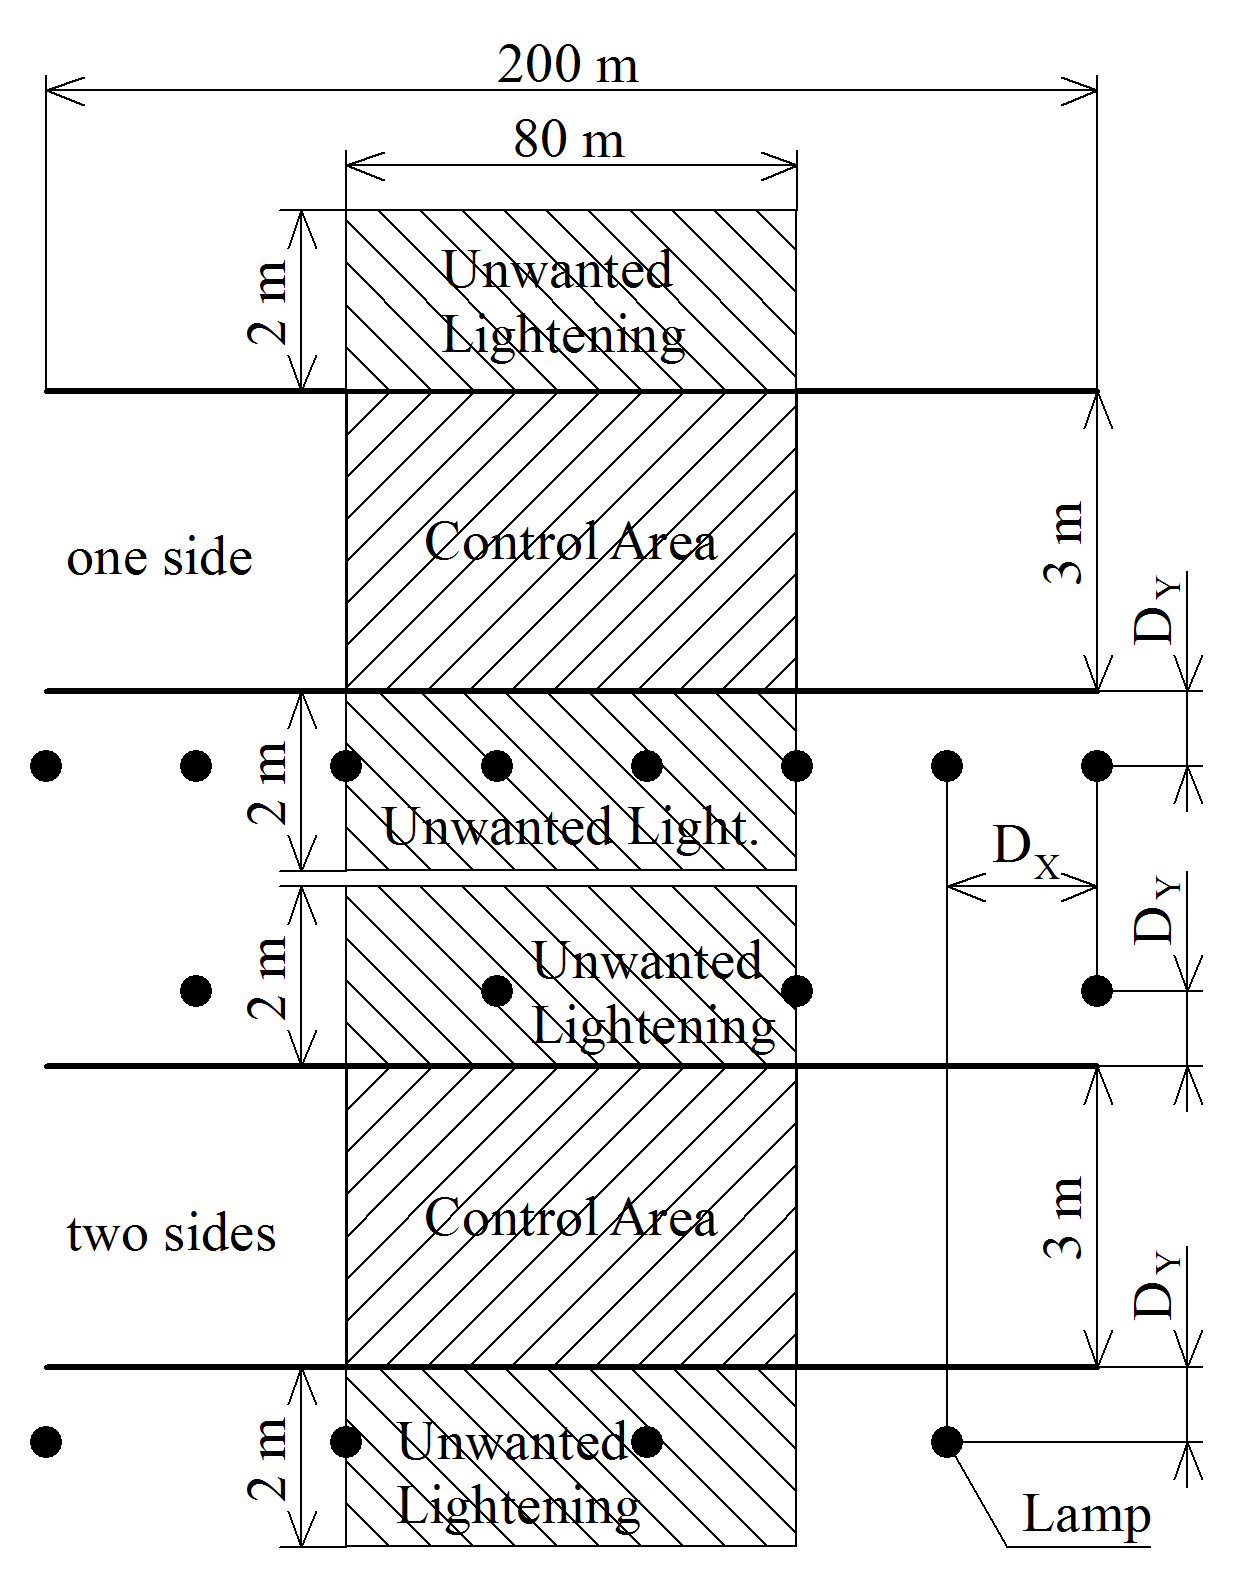
\includegraphics[width=0.8\columnwidth]{kotyChodniku}
  \caption{Dimensions of studied sidewalks}
  \label{fig:sidewalk}
\end{figure}

There was used one point crossover in the genetic algorithm. The probability of crossovers was set to 80~\% and mutation was set to 5~\%. Both the parent population size and offspring size were 200. The calculations were finished after 60 births. All these settings were set after several testing to get smooth and fast calculation of the algorithm.

\subsection{Fitness function}
Suitable fitness function is the key factor for genetic evaluation. This function is used for determination which results are better than others. It is set up by knowing the target behavior of the result in common cases. However there is no cookbook which would define how to create such function.

Authors decided to create several weights $w\left(x\right)$ based on exponential function and these rules multiply one with each other to get resulting fitness function. The basic function was defined by the formula:

\begin{equation}
w\left(x\right)= e^{-a\cdot x}
\label{eq:rule}
\end{equation}

where:
\begin{description}
\item [$x$...] is current result and
\item [$a$...] is parameter which defines the slope (first derivation) of the function.
\end{description}

There were several reasons to choose the (\ref{eq:rule}). However the main advantage is that the function is equal to 1 at zero and the limit at infinity is equal to zero. The specific weights were defined as follow:

\begin{equation}
w_1\left(E_{min}\right)= \left\{
  \begin{array}{l l}
    e^{10 \cdot (E_{min} - E_{minT})} & E_{min} \in \left\langle 0, E_{minT}\right\rangle\\
    e^{(E_{minT}-E_{min})/10} & E_{min} \in \left( E_{minT}, \infty\right)
  \end{array}\right.
\label{eq:weightEmin}
\end{equation}

\begin{equation}
w_2\left(\overline{E}\right)= \left\{
  \begin{array}{l l}
    e^{\overline{E} - \overline{E}_{T}} & \overline{E} \in \left\langle 0, \overline{E}_{T}\right\rangle\\
    e^{\overline{E}_{T} -\overline{E}} & \overline{E} \in \left( \overline{E}_{T}, \infty\right)
  \end{array}\right.
\label{eq:weightEavg}
\end{equation}

\begin{equation}
w_3\left(\overline{E}_o\right)= e^{\overline{E}_o/100}
\label{eq:weightEo}
\end{equation}

\subsection{Elitism}